% =====================================================================
%  Smart LLM Router: A Free-First, Cost-Aware Gateway for LLM Requests
%  Author: Abhilash Shishodia
%
%  Compile with:  pdflatex smart_llm_router.tex   (run twice for refs)
%  Self-contained: uses TikZ for figures (no external image files).
% =====================================================================
\documentclass[11pt]{article}

\usepackage[utf8]{inputenc}
\usepackage[T1]{fontenc}
\usepackage[margin=1in]{geometry}
\usepackage{amsmath,amssymb}
\usepackage{graphicx}
\usepackage{booktabs}
\usepackage{xcolor}
\usepackage{url}
\usepackage{tikz}
\usetikzlibrary{arrows.meta,positioning,shapes.geometric}
\usepackage[hidelinks]{hyperref}
\usepackage{authblk}
\usepackage{microtype}
\setlength{\emergencystretch}{2em}

% ---- title ----------------------------------------------------------
\title{\textbf{Smart LLM Router: A Free-First, Cost-Aware Gateway\\
for Routing Coding Assistance Between Free and Paid Language Models}}

\author[]{Abhilash Shishodia}
\affil[]{\texttt{Independent Researcher}}
\date{\today}

% ---- convenience macros --------------------------------------------
\newcommand{\cfree}{c_{\mathrm{free}}}
\newcommand{\cpaid}{c_{\mathrm{paid}}}
\newcommand{\Qt}{Q_{\mathrm{target}}}

\begin{document}
\maketitle

\begin{abstract}
Premium AI coding assistants built on frontier large language models (LLMs)
deliver excellent quality but charge per token, so cost scales with usage even
though a large fraction of everyday developer requests---autocompletion,
boilerplate generation, and short explanations---do not require a frontier
model. We present the \emph{Smart LLM Router}, a free-first, cost-aware gateway
that classifies each incoming request, serves it with a free or local model by
default, and escalates to a paid model only when the task is predicted to be
hard or when a lightweight verifier judges the free response to be inadequate.
The router exposes a drop-in, OpenAI-compatible interface, so existing IDE and
CLI clients need no changes. We formalize the routing problem as constrained
cost minimization subject to a quality floor, describe a \emph{classify--route
--verify} pipeline with a confidence-based escalation loop, and present an
analytic cost model showing that expected spend is proportional to the fraction
of requests that ultimately reach a paid tier. We report a preliminary
empirical study on a 44-problem coding suite with executable unit tests, using
\emph{small locally-running (free) models} and \emph{large cloud-based models}
that are comparable in capability to paid-tier hosted models; evaluating true
metered paid APIs is left as future work. On the hardest problems small local
models solve far fewer tasks than large models, yet the router---by keeping
easy requests free and escalating only when a verifier flags a failure---matches
the strong model's task-success rate while sending only a fraction of requests
to the large tier. We also provide a reproducible evaluation protocol (datasets,
metrics, baselines, and ablations) for larger-scale validation.
We situate the design against existing routers and gateways
(e.g., RouteLLM, LiteLLM, OpenRouter, Not Diamond) and highlight its
distinguishing combination of free-first defaults, automatic escalation,
local-privacy routing, and per-request budget guardrails.
\end{abstract}

\noindent\textbf{Keywords:} LLM routing, model cascades, cost-aware inference,
AI gateway, code assistants, model selection.

% =====================================================================
\section{Introduction}
\label{sec:intro}
Large language models (LLMs), built on the transformer
architecture~\cite{attention}, have become a standard part of the
software-development workflow, powering code completion, refactoring, test
generation, debugging, and natural-language explanation of code. The strongest of these assistants are
backed by frontier models offered under metered, per-token pricing. While the
quality is high, the cost structure is unfavorable for teams: spend grows
linearly with usage, bills are difficult to predict, and---crucially---the
\emph{same} premium price is paid for trivial and hard requests alike.

Two empirical observations motivate this work. First, the difficulty
distribution of real developer requests is highly skewed: many requests are
easy (rename a symbol, explain a function, generate a small stub) and a
minority are genuinely hard (design a scalable architecture, reason about a
subtle concurrency bug, perform a security-sensitive refactor). Second, the
capability gap between free/open and premium models has narrowed substantially
for easy tasks, so a cheaper model often produces an answer indistinguishable
from a frontier model on such requests. Together these imply that routing every
request to a frontier model overspends on the easy majority.

We propose the \textbf{Smart LLM Router}: a gateway that sits between the client
(IDE or CLI) and a pool of model providers and \emph{automatically decides,
per request, whether a free/local model suffices or a paid model is warranted}.
The router is \emph{free-first}: it defaults to zero-marginal-cost models and
escalates to paid tiers only on demand. Escalation is driven both by a
\emph{predictive} signal (a complexity classifier applied before generation)
and a \emph{reactive} signal (a verifier that grades the free answer and
triggers re-routing when confidence is low). The interface is
OpenAI-compatible, so adoption requires no client changes.

\paragraph{Contributions.}
\begin{itemize}
  \item We formalize free-first coding-assistant routing as constrained cost
        minimization subject to a quality floor (Section~\ref{sec:decision}).
  \item We describe a \emph{classify--route--verify} architecture with an
        invisible escalation loop and per-request budget guardrails
        (Sections~\ref{sec:system}--\ref{sec:decision}).
  \item We derive an analytic cost model that expresses expected spend and
        relative savings in terms of the effective paid-routing fraction
        (Section~\ref{sec:cost}).
  \item We contribute a concrete, reproducible evaluation protocol for
        software-engineering workloads (Section~\ref{sec:eval}).
  \item We position the design against existing routers and gateways and
        articulate what it uniquely combines (Section~\ref{sec:related}).
\end{itemize}

% =====================================================================
\section{Background and Related Work}
\label{sec:related}
\paragraph{Model cascades and cost-aware inference.}
Routing simpler queries to cheaper models is an established idea.
FrugalGPT~\cite{frugalgpt} introduced LLM cascades that call models in
increasing order of cost and stop early when a scorer deems an answer adequate.
RouteLLM~\cite{routellm} learns a binary router between a strong and a weak
model from human-preference data, reporting up to $85\%$ cost reduction while
retaining roughly $95\%$ of GPT-4 quality on common benchmarks, and provides a
drop-in OpenAI-compatible server with threshold calibration.
Hybrid LLM~\cite{hybridllm} similarly learns quality-aware query routing
between a small and a large model. AutoMix~\cite{automix} mixes models using
self-verification to decide when to escalate. Our design draws on both the
predictive routing of RouteLLM/Hybrid~LLM and the reactive, verify-then-escalate
cascade of FrugalGPT/AutoMix, but frames them within a \emph{free-first},
multi-tier, privacy- and budget-aware gateway targeted at coding workloads.

\paragraph{Gateways and hosted routers.}
LiteLLM~\cite{litellm} is an open-source AI gateway exposing an
OpenAI-compatible API to 100+ providers with fallbacks, load-balancing, and
spend tracking, but its routing is primarily rule- and fallback-based rather
than quality-aware. OpenRouter~\cite{openrouter} is a hosted unified API to many
models (including free ones) with automatic and price-based routing. Portkey~
\cite{portkey} is an AI gateway with routing, caching, guardrails, and
observability. Not Diamond~\cite{notdiamond}, Martian~\cite{martian}, and
Unify~\cite{unify} are hosted services that select a model per query to optimize
cost, quality, and latency. Semantic Router~\cite{semanticrouter} is an
open-source decision layer that routes by embedding similarity (intent), not by
predicted difficulty or cost.

\paragraph{Local serving.}
Free-first routing is enabled by efficient local inference. Systems such as
vLLM~\cite{vllm} and packagers such as Ollama~\cite{ollama} make it practical to
serve capable open models (e.g., code-specialized models) on local hardware at
zero marginal cost and with data locality.

\paragraph{Code benchmarks.}
Our evaluation follows the lineage of standard code-generation benchmarks that
grade models by executing generated programs against unit tests:
HumanEval~\cite{humaneval} and MBPP~\cite{mbpp} for function-level synthesis,
BigCodeBench~\cite{bigcodebench} for more realistic library usage,
LiveCodeBench~\cite{livecodebench} for contamination-resistant, continuously
updated problems, and SWE-bench~\cite{swebench} for repository-level issue
resolution. We adopt the same execution-based, \emph{pass@1} methodology on a
compact suite spanning five difficulty tiers (Section~\ref{sec:eval}).

\paragraph{Positioning.}
Table~\ref{tab:landscape} summarizes representative systems. Relative to prior
work, the Smart LLM Router's distinguishing feature is not a single new
mechanism but a \emph{combination}: free/local defaults, \emph{both} predictive
and reactive escalation to paid tiers, explicit privacy-based routing of
sensitive code to local-only models, and hard per-request/per-period budget
guardrails---delivered behind one drop-in gateway.

\begin{table}[t]
\centering
\small
\caption{Representative routers and gateways. ``Quality-aware'' means routing
uses a learned or verified estimate of answer quality rather than only static
rules.}
\label{tab:landscape}
\begin{tabular}{@{}lllcc@{}}
\toprule
System & Type & Hosting & Quality-aware & Open source \\
\midrule
RouteLLM~\cite{routellm}          & Router framework   & Self-host   & Yes & Yes \\
FrugalGPT~\cite{frugalgpt}        & Cascade            & Self-host   & Yes & Partial \\
Hybrid LLM~\cite{hybridllm}       & Router             & Self-host   & Yes & Partial \\
LiteLLM~\cite{litellm}            & Gateway            & Self-host   & No  & Yes \\
OpenRouter~\cite{openrouter}      & Unified API/router & Hosted      & Partial & No \\
Portkey~\cite{portkey}            & Gateway            & Both        & Partial & Partial \\
Not Diamond~\cite{notdiamond}     & Router             & Hosted      & Yes & No \\
Semantic Router~\cite{semanticrouter} & Decision layer & Self-host   & No  & Yes \\
\textbf{Smart LLM Router (ours)}  & Free-first gateway & Self-host   & Yes & --- \\
\bottomrule
\end{tabular}
\end{table}

% =====================================================================
\section{System Design}
\label{sec:system}
The router is a stateless service exposing an OpenAI-compatible
\texttt{/chat/completions} endpoint. Each request passes through a short
\emph{classify--route--verify} pipeline (Figure~\ref{fig:arch}).

\begin{enumerate}
  \item \textbf{Classify.} A fast complexity estimator maps the request (prompt,
        task type, context size, attached files) to a scalar difficulty score
        $x(q)\in[0,1]$. The estimator can be rule-based, embedding-based, or a
        small fine-tuned classifier; these can be combined.
  \item \textbf{Route.} A policy $\pi$ selects the cheapest model tier whose
        predicted quality satisfies the caller's quality floor, subject to
        privacy and budget constraints.
  \item \textbf{Verify.} For a request served by a lower tier, a lightweight
        verifier $v(\cdot)$ grades the response. If confidence is below a
        threshold $\delta$, the request is transparently re-routed (escalated)
        to the next tier. The client observes only the final answer.
\end{enumerate}

Auxiliary services support the pipeline: a response \emph{cache} avoids paying
twice for identical requests; a \emph{cost/usage ledger} records per-request
spend for budgeting and analytics; and a \emph{policy configuration} declares
thresholds, budgets, and privacy rules.

\begin{figure}[t]
\centering
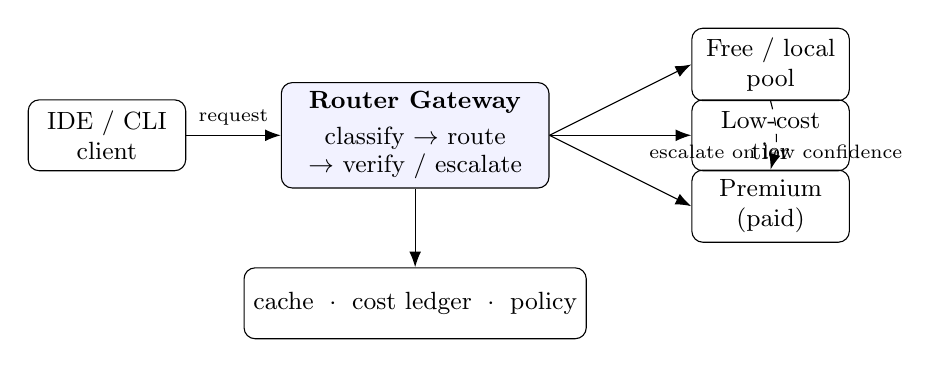
\begin{tikzpicture}[
  node distance=8mm and 12mm,
  box/.style={draw, rounded corners, align=center, minimum height=9mm,
              minimum width=20mm, font=\small},
  gw/.style ={draw, rounded corners, align=center, fill=blue!5,
              minimum width=34mm, font=\small},
  every edge/.style={draw, -{Latex[length=2mm]}}
]
\node[box] (client) {IDE / CLI\\client};
\node[gw, right=of client] (gateway) {\textbf{Router Gateway}\\[2pt]
      classify $\to$ route\\[-1pt] $\to$ verify / escalate};
\node[box, right=18mm of gateway, yshift=9mm]  (free) {Free / local\\pool};
\node[box, right=18mm of gateway]              (low)  {Low-cost\\tier};
\node[box, right=18mm of gateway, yshift=-9mm] (paid) {Premium\\(paid)};

\draw (client) edge node[above,font=\scriptsize]{request} (gateway);
\draw (gateway.east) edge (free.west);
\draw (gateway.east) edge (low.west);
\draw (gateway.east) edge (paid.west);

\draw[dashed, -{Latex[length=2mm]}] (free.south) to[bend left=15]
      node[below,font=\scriptsize]{escalate on low confidence} (paid.north);

\node[box, below=10mm of gateway, minimum width=34mm] (aux)
     {cache \(\;\cdot\;\) cost ledger \(\;\cdot\;\) policy};
\draw[<->] (gateway) edge (aux);
\end{tikzpicture}
\caption{The Smart LLM Router. Requests are classified, routed to the cheapest
adequate tier, and---if the free/low-cost answer fails verification---
transparently escalated to a paid tier. Auxiliary services provide caching,
cost accounting, and policy.}
\label{fig:arch}
\end{figure}

% =====================================================================
\section{The Decision Engine}
\label{sec:decision}
\subsection{Problem formulation}
Let a query be $q$ drawn from workload distribution $\mathcal{D}$. Let the model
pool be organized into $K$ tiers $T_1,\dots,T_K$ ordered by increasing cost,
with per-request cost $c_k$ (with $c_1=\cfree\approx 0$ for the free/local tier)
and a quality function $Q_k(q)\in[0,1]$ giving the (expected) quality of tier
$k$ on query $q$. A router is a policy $\pi$ that maps observable request
features to a tier (and possibly a sequence of tiers via escalation). We seek to
minimize expected cost subject to a quality floor $\Qt$:
\begin{equation}
\min_{\pi}\;\; \mathbb{E}_{q\sim\mathcal{D}}\big[\,C_\pi(q)\,\big]
\quad\text{s.t.}\quad
\mathbb{E}_{q\sim\mathcal{D}}\big[\,Q_\pi(q)\,\big]\;\ge\;\Qt ,
\label{eq:opt}
\end{equation}
where $C_\pi(q)$ and $Q_\pi(q)$ are the realized cost and quality of the policy
on $q$. Introducing a multiplier $\lambda\ge0$ yields the unconstrained
surrogate
\begin{equation}
\min_{\pi}\;\;\mathbb{E}_{q}\big[\,C_\pi(q)\,-\,\lambda\,Q_\pi(q)\,\big],
\label{eq:lagrangian}
\end{equation}
so that $\lambda$ trades cost against quality; it is the analogue of RouteLLM's
calibrated cost threshold~\cite{routellm}.

\subsection{Predictive routing signals}
Before generation, the router combines several signals into the difficulty
score $x(q)$ and side constraints:
\begin{itemize}
  \item \textbf{Task type.} Autocompletion, boilerplate, and short explanations
        bias toward free tiers; architecture, security, and multi-file
        debugging bias toward paid tiers.
  \item \textbf{Predicted complexity.} A classifier or heuristics estimate
        difficulty from the prompt and repository context.
  \item \textbf{Context size.} Very long contexts favor a capable tier able to
        use them effectively.
  \item \textbf{Privacy flag.} Requests touching sensitive code set a hard
        constraint $\pi(q)\in\{\text{local tiers}\}$.
  \item \textbf{Budget guardrail.} A remaining-budget state $b$ caps paid usage
        over a period; when $b$ is exhausted, paid tiers are disabled.
\end{itemize}
For a two-tier (free/paid) instantiation with threshold $\tau$, the predictive
rule is
\begin{equation}
r_{\mathrm{pred}}(q)=
\begin{cases}
\text{paid}, & x(q)\ge\tau \ \text{ and privacy/budget allow},\\
\text{free}, & \text{otherwise.}
\end{cases}
\label{eq:predrule}
\end{equation}

\subsection{Reactive escalation}
When a request is served by the free tier, the verifier produces a confidence
score $v(a,q)\in[0,1]$ for answer $a$ (e.g., self-consistency, unit-test
execution for code, a small critic model, or format/lint checks). If
$v(a,q)<\delta$, the request escalates to the paid tier. Escalation is invisible
to the client. The verifier is the crux of the system: an over-eager verifier
wastes escalations, while a lax one degrades quality.

% =====================================================================
\section{Cost Model}
\label{sec:cost}
Consider the two-tier instantiation with $\cfree\approx0$. Let
\begin{equation}
p \;=\; \underbrace{\Pr\!\big[x(q)\ge\tau\big]}_{\text{routed paid directly}}
\;+\;
\underbrace{\Pr\!\big[x(q)<\tau\big]\,\Pr\!\big[v(a,q)<\delta \mid \text{free}\big]}_{\text{escalated after verify}}
\label{eq:p}
\end{equation}
be the \emph{effective paid fraction}: the probability that a request ultimately
consumes the paid tier. Ignoring the small cost of local generation and
verification, the expected cost per request is
\begin{equation}
\mathbb{E}[C] \;=\; p\,\cpaid ,
\label{eq:ecost}
\end{equation}
whereas the all-paid baseline costs $\cpaid$ per request. The relative saving is
therefore
\begin{equation}
\mathrm{Savings} \;=\; 1 - p .
\label{eq:savings}
\end{equation}
Equation~\eqref{eq:savings} makes the design goal explicit: \emph{minimize the
effective paid fraction $p$ without violating the quality floor}. Lowering
$\tau$ or $\delta$ reduces $p$ (more savings) but risks quality; the multiplier
$\lambda$ in Eq.~\eqref{eq:lagrangian} sets the operating point.

For the general $K$-tier cascade with escalation probabilities, the expected
cost telescopes as
\begin{equation}
\mathbb{E}[C] \;=\; \sum_{k=1}^{K} c_k \, \rho_k ,
\qquad
\rho_k \;=\; \Pr[\text{tier }k\text{ is invoked}],
\label{eq:kcost}
\end{equation}
where $\rho_k$ is determined by the routing thresholds and the per-tier
escalation rates. A worked illustration: if $75\%$ of requests are served for
free and never escalate, and the remaining $25\%$ reach the paid tier at
$\cpaid\!\approx\!\$0.03$ per request, then $p=0.25$ and expected spend is
$\$0.0075$ per request---about a $75\%$ reduction versus all-paid. These
figures are illustrative; realized savings depend on the workload's difficulty
distribution and verifier accuracy, which motivates the evaluation below.

% =====================================================================
\section{Empirical Evaluation}
\label{sec:empirical}
We report a preliminary study that instantiates the router and measures both the
capability gap it exploits and its end-to-end behavior.

\subsection{Setup}
We implement the gateway as a stateless service backed by
Ollama~\cite{ollama}. We evaluate two model classes, using deliberately honest
labels:
\begin{itemize}
  \item \textbf{Small local free models} run locally at zero marginal cost and
        are always available offline: \texttt{llama3.2} (3B), \texttt{gemma3},
        and \texttt{phi4-mini}.
  \item \textbf{Large cloud-based models} are large models served from Ollama's
        cloud that are comparable in capability to paid-tier hosted models:
        \texttt{gpt-oss:120b} and \texttt{qwen3-coder:480b}. We do \emph{not}
        evaluate metered commercial paid APIs; extending the study to true paid
        tiers is future work.
\end{itemize}
Our workload is a suite of $44$ Python programming problems spanning five
difficulty tiers (easy, medium, hard, expert, and ``brutal''), each with hidden
unit tests. We grade with execution-based \emph{pass@1}: a task counts as solved
if the model's generated function passes all its tests, run in an isolated
subprocess with a timeout. In these experiments the reactive verifier executes
the task's unit tests, i.e., it is an \emph{oracle} verifier; realistic
deployment verifiers (generated tests, self-consistency, critic models) are
weaker, so our escalation results are an \emph{upper bound} on what reactive
verification recovers. Reported dollar figures use the configurable, illustrative
pricing of Section~\ref{sec:cost}, not vendor prices.

\subsection{Capability gap between model classes}
Table~\ref{tab:bench} reports per-tier pass@1 for each model on the full suite.
The pattern that motivates free-first routing is clear: on easy and medium
problems the small local models are competitive with the large models, but on
the hardest (``brutal'') tier they fall well behind---averaging $47\%$ versus
$96\%$ for the large cloud models---so difficulty-aware routing has real headroom.

\begin{table}[t]
\centering
\small
\caption{Execution-based pass@1 on the 44-problem suite (higher is better).
Small local free models match large models on easy work but lag sharply on the
hardest tier, which is exactly what a difficulty-aware router can exploit.}
\label{tab:bench}
\begin{tabular}{@{}llcccccc@{}}
\toprule
Model & Class & Overall & Easy & Med. & Hard & Exp. & Brutal \\
\midrule
\texttt{llama3.2} (3B)      & small local free & 73\% & 100\% & 100\% & 100\% & 58\%  & 42\%  \\
\texttt{gemma3}             & small local free & 93\% & 100\% & 100\% & 88\%  & 100\% & 83\%  \\
\texttt{phi4-mini}          & small local free & 52\% & 100\% & 88\%  & 75\%  & 33\%  & 17\%  \\
\midrule
\texttt{gpt-oss:120b}       & large cloud      & 100\%& 100\% & 100\% & 100\% & 100\% & 100\% \\
\texttt{qwen3-coder:480b}   & large cloud      & 98\% & 100\% & 100\% & 100\% & 100\% & 92\%  \\
\midrule
\emph{avg small local free} &                  & 73\% &       &       &       &       & 47\%  \\
\emph{avg large cloud}      &                  & 99\% &       &       &       &       & 96\%  \\
\bottomrule
\end{tabular}
\end{table}

\subsection{Router effectiveness}
\label{sec:router-results}
We run the four strategies of Section~\ref{sec:decision} on the same suite with
\texttt{llama3.2} as the small local (free) tier and \texttt{gpt-oss:120b} as the
large cloud tier, threshold $\tau{=}0.45$.
Table~\ref{tab:router} summarizes the outcome. Always-free solves only the easy
majority; always-cloud solves everything at full cost. The router
\emph{matches the large model's task-success rate} while routing a substantial
share of requests to the free tier, because the reactive (oracle) verifier
catches cases the predictive classifier under-rated and escalates only those.
Consistent with Eq.~\eqref{eq:savings}, realized cost tracks the effective
paid fraction $p$. Six requests were escalated after a silent local failure
(e.g., regular-expression matching, the parenthetical calculator, and
decode-string), and all six were recovered by the large model---directly
illustrating the value of reactive verification.

\begin{table}[t]
\centering
\small
\caption{Router versus baselines on the 44-problem suite (small local tier
\texttt{llama3.2}; large cloud tier \texttt{gpt-oss:120b}; $\tau{=}0.45$). The
router matches the large model's pass@1 while sending only $52\%$ of requests to
the large cloud tier. Cost uses the illustrative pricing of
Section~\ref{sec:cost}, not vendor prices.}
\label{tab:router}
\begin{tabular}{@{}lccccc@{}}
\toprule
Strategy & pass@1 & Cloud frac.\ $p$ & Cost & Avg.\ latency & Savings \\
\midrule
Always free (local)    & 80\%  & 0\%   & \$0.0000 & 2.41\,s & 100\% \\
Always cloud (baseline)& 100\% & 100\% & \$0.0491 & 4.06\,s & 0\% \\
Random                 & 84\%  & 41\%  & \$0.0194 & 3.04\,s & 61\% \\
\textbf{Router (ours)} & \textbf{100\%} & 52\% & \$0.0287 & 3.80\,s & \textbf{41\%} \\
\bottomrule
\end{tabular}
\end{table}

% =====================================================================
\section{Proposed Larger-Scale Evaluation}
\label{sec:eval}
Our study above is small and uses an oracle verifier; we outline a fuller
protocol for community-scale validation.

\paragraph{Datasets and workloads.}
(i)~Code generation: HumanEval~\cite{humaneval} and MBPP~\cite{mbpp};
(ii)~repository-level tasks: SWE-bench~\cite{swebench};
(iii)~general instruction quality: MT-Bench~\cite{mtbench};
(iv)~a de-identified trace of real developer requests to reflect the true
difficulty distribution and task mix.

\paragraph{Metrics.}
For each system we report: expected cost per request and total spend; the
effective paid fraction $p$; task quality (\textit{pass@}$k$ for code;
LLM-judge win-rate versus a frontier reference for open-ended tasks);
escalation rate and escalation precision/recall; added end-to-end latency
(routing plus verification overhead); and cache hit rate.

\paragraph{Baselines.}
Always-paid (upper cost bound), always-free (lower cost bound), random routing,
RouteLLM~\cite{routellm} (mf router), and a FrugalGPT-style cascade
\cite{frugalgpt}. Reporting cost--quality curves (quality versus spend as $\tau,
\delta$ vary) enables Pareto comparison rather than single-point claims.

\paragraph{Ablations.}
(i)~classifier versus pure heuristics for $x(q)$;
(ii)~with and without the reactive verifier;
(iii)~verifier variants (unit-test execution, self-consistency, critic model);
(iv)~effect of budget guardrails; and
(v)~sensitivity to the free-tier model choice.

\paragraph{Hypotheses.}
\textbf{H1:} free-first routing attains a strictly better cost--quality Pareto
frontier than always-paid on realistic coding traces.
\textbf{H2:} reactive verification recovers most of the quality lost by
aggressive predictive routing at modest additional cost.
\textbf{H3:} the dominant cost driver is the effective paid fraction $p$, as
predicted by Eq.~\eqref{eq:savings}.

% =====================================================================
\section{Discussion, Limitations, and Ethics}
\label{sec:discussion}
\paragraph{Limitations.}
The system's savings and quality hinge on the verifier and classifier; both can
be miscalibrated or drift as workloads change, requiring periodic
recalibration. Routing and verification add latency, which must stay small
relative to generation time. Free API tiers impose rate limits and may change
terms; local models require adequate hardware. Benchmark contamination and the
non-stationarity of hosted models complicate reproducibility; we therefore
emphasize cost--quality \emph{curves} and pinned model versions.

\paragraph{Ethical and practical considerations.}
Free-first routing can lower the cost and energy footprint of AI assistance and,
via local-only routing of sensitive code, improve data locality and privacy.
Conversely, mis-routing risks silently degrading answer quality; transparent
logging of which tier served each request, along with user-visible controls,
mitigates this. Budget guardrails prevent runaway spend but must not be used to
degrade service without disclosure.

% =====================================================================
\section{Conclusion}
\label{sec:conclusion}
We presented the Smart LLM Router, a free-first, cost-aware gateway that routes
coding-assistance requests to free or local models by default and escalates to
paid models only when predicted difficulty or verified low confidence warrants
it. We formalized routing as constrained cost minimization, described a
classify--route--verify architecture with transparent escalation, derived a
cost model in which expected spend is proportional to the effective paid
fraction, and proposed a reproducible evaluation protocol. We hope this design
and protocol help teams obtain most of the benefit of frontier coding
assistants at a fraction of the cost, while retaining privacy and predictable
budgets.

% =====================================================================
\begin{thebibliography}{99}
\small

\bibitem{routellm}
I.~Ong, A.~Almahairi, V.~Wu, W.-L.~Chiang, T.~Wu, J.~E.~Gonzalez,
M.~W.~Kadous, and I.~Stoica.
\newblock RouteLLM: Learning to Route LLMs with Preference Data.
\newblock \emph{arXiv:2406.18665}, 2024. \url{https://arxiv.org/abs/2406.18665}

\bibitem{frugalgpt}
L.~Chen, M.~Zaharia, and J.~Zou.
\newblock FrugalGPT: How to Use Large Language Models While Reducing Cost and
Improving Performance.
\newblock \emph{arXiv:2305.05176}, 2023. \url{https://arxiv.org/abs/2305.05176}

\bibitem{hybridllm}
D.~Ding, A.~Mallick, C.~Wang, R.~Sim, S.~Mukherjee, V.~R\"uhle,
L.~V.~S.~Lakshmanan, and A.~H.~Awadallah.
\newblock Hybrid LLM: Cost-Efficient and Quality-Aware Query Routing.
\newblock \emph{International Conference on Learning Representations (ICLR)},
2024. \url{https://arxiv.org/abs/2404.14618}

\bibitem{automix}
A.~Madaan, P.~Aggarwal, A.~Anand, et~al.
\newblock AutoMix: Automatically Mixing Language Models.
\newblock \emph{arXiv:2310.12963}, 2023. \url{https://arxiv.org/abs/2310.12963}

\bibitem{vllm}
W.~Kwon, Z.~Li, S.~Zhuang, Y.~Sheng, L.~Zheng, C.~H.~Yu, J.~E.~Gonzalez,
H.~Zhang, and I.~Stoica.
\newblock Efficient Memory Management for Large Language Model Serving with
PagedAttention.
\newblock \emph{ACM Symposium on Operating Systems Principles (SOSP)}, 2023.
\url{https://arxiv.org/abs/2309.06180}

\bibitem{humaneval}
M.~Chen, J.~Tworek, H.~Jun, et~al.
\newblock Evaluating Large Language Models Trained on Code.
\newblock \emph{arXiv:2107.03374}, 2021. \url{https://arxiv.org/abs/2107.03374}

\bibitem{mbpp}
J.~Austin, A.~Odena, M.~Nye, et~al.
\newblock Program Synthesis with Large Language Models.
\newblock \emph{arXiv:2108.07732}, 2021. \url{https://arxiv.org/abs/2108.07732}

\bibitem{swebench}
C.~E.~Jimenez, J.~Yang, A.~Wettig, S.~Yao, K.~Pei, O.~Press, and K.~Narasimhan.
\newblock SWE-bench: Can Language Models Resolve Real-World GitHub Issues?
\newblock \emph{ICLR}, 2024. \url{https://arxiv.org/abs/2310.06770}

\bibitem{livecodebench}
N.~Jain, K.~Han, A.~Gu, W.-D.~Li, F.~Yan, T.~Zhang, S.~Wang, A.~Solar-Lezama,
K.~Sen, and I.~Stoica.
\newblock LiveCodeBench: Holistic and Contamination-Free Evaluation of Large
Language Models for Code.
\newblock \emph{arXiv:2403.07974}, 2024. \url{https://arxiv.org/abs/2403.07974}

\bibitem{bigcodebench}
T.~Y.~Zhuo, M.~C.~Vu, J.~Chim, et~al.
\newblock BigCodeBench: Benchmarking Code Generation with Diverse Function Calls
and Complex Instructions.
\newblock \emph{arXiv:2406.15877}, 2024. \url{https://arxiv.org/abs/2406.15877}

\bibitem{mtbench}
L.~Zheng, W.-L.~Chiang, Y.~Sheng, et~al.
\newblock Judging LLM-as-a-Judge with MT-Bench and Chatbot Arena.
\newblock \emph{NeurIPS Datasets and Benchmarks}, 2023.
\url{https://arxiv.org/abs/2306.05685}

\bibitem{litellm}
BerriAI.
\newblock LiteLLM: Python SDK and Proxy Server (AI Gateway) to call 100+ LLM
APIs in OpenAI format.
\newblock Software, accessed 2026. \url{https://github.com/BerriAI/litellm}

\bibitem{openrouter}
OpenRouter.
\newblock A unified API and marketplace for LLMs with model routing.
\newblock Accessed 2026. \url{https://openrouter.ai}

\bibitem{portkey}
Portkey.
\newblock AI Gateway: routing, caching, guardrails, and observability for LLMs.
\newblock Accessed 2026. \url{https://portkey.ai}

\bibitem{notdiamond}
Not Diamond.
\newblock An AI model router that selects the best model per query.
\newblock Accessed 2026. \url{https://www.notdiamond.ai}

\bibitem{martian}
Martian.
\newblock Model router for cost- and quality-aware LLM selection.
\newblock Accessed 2026. \url{https://www.withmartian.com}

\bibitem{unify}
Unify.
\newblock Routing and benchmarking across LLM providers via a single API.
\newblock Accessed 2026. \url{https://unify.ai}

\bibitem{semanticrouter}
Aurelio AI.
\newblock Semantic Router: a fast decision layer for LLMs and agents.
\newblock Software, accessed 2026.
\url{https://github.com/aurelio-labs/semantic-router}

\bibitem{ollama}
Ollama.
\newblock Run open large language models locally.
\newblock Accessed 2026. \url{https://ollama.com}

\bibitem{attention}
A.~Vaswani, N.~Shazeer, N.~Parmar, J.~Uszkoreit, L.~Jones, A.~N.~Gomez,
{\L}.~Kaiser, and I.~Polosukhin.
\newblock Attention Is All You Need.
\newblock \emph{Advances in Neural Information Processing Systems (NeurIPS)},
2017. \url{https://arxiv.org/abs/1706.03762}

\end{thebibliography}

\end{document}
